\documentclass[11pt,a4paper]{article}

\usepackage[utf8]{inputenc}
\usepackage[T1]{fontenc}
\usepackage{lmodern}
\usepackage[margin=2.5cm]{geometry}
\usepackage{amsmath,amssymb}
\usepackage{booktabs}
\usepackage{graphicx}
\usepackage{float}
\usepackage{caption}
\usepackage{subcaption}
\usepackage{xcolor}
\usepackage{hyperref}

\graphicspath{{report_2/}}

\hypersetup{
    colorlinks=true,
    linkcolor=blue!50!black,
    urlcolor=blue!50!black,
    citecolor=blue!50!black
}

\title{\vspace{3cm}\textbf{\LARGE Data Exploration and Analytics: Assignment 03}\\[0.4em]
\large Dimension Reduction Methods on Forty Soybean Cultivars from Subsequent Harvests}
\author{Claudia Rodr\'iguez Lorenzo, Leire Guevara Rom\'an, V\'ictor Mu\~noz Cuadrado}
\date{November 25, 2026}

\begin{document}

\maketitle
\vspace{0.6cm}
\begin{abstract}
\noindent
This report presents a Principal Component Analysis (PCA) of the \textit{Forty Soybean Cultivars from Subsequent Harvests} dataset ($n = 320$ observations). Following the assignment instructions, the target variable Grain Yield (\texttt{GY}) and the experimental design identifiers (\texttt{Season}, \texttt{Cultivar}, \texttt{Repetition}) are omitted, leaving 7 continuous agronomic features (\texttt{PH}, \texttt{IFP}, \texttt{NLP}, \texttt{NGP}, \texttt{NGL}, \texttt{NS}, and \texttt{MHG}). Using Python (\texttt{script.py}), two separate PCA analyses are performed and compared: first using the sample covariance matrix (on mean-centered variables) and second using the Pearson correlation matrix (on standardized variables). For each method, we examine the matrix structure, eigenvalues, explained variance thresholds (90\%, 95\%, and 99\%), scree plots, eigenvectors, factor loadings, mathematical equations of the first three principal components, and 2D and 3D component projections.
\end{abstract}

\newpage
\tableofcontents
\newpage

\section{Dataset Overview and Selected Features}

The dataset \textit{Forty Soybean Cultivars from Subsequent Harvests} (\texttt{data.csv}) contains 320 observations from an agricultural experiment evaluating 40 soybean cultivars across 2 consecutive seasons and 4 repetitions. To perform dimension reduction on the explanatory traits without target leakage, the target variable \textbf{Grain Yield (\texttt{GY})} and the categorical design factors (\texttt{Season}, \texttt{Cultivar}, \texttt{Repetition}) are excluded.

Table~\ref{tab:dataset} summarizes the 7 quantitative predictor variables included in both PCA analyses, along with their sample means ($\bar{x}$), standard deviations ($s$), and sample variances ($s^2$).

\begin{table}[H]
\centering
\caption{Descriptive statistics of the 7 continuous soybean features ($n = 320$).}
\label{tab:dataset}
\begin{tabular}{llrrr}
\toprule
\textbf{Variable} & \textbf{Description} & \textbf{Mean ($\bar{x}$)} & \textbf{Std.\ Dev.\ ($s$)} & \textbf{Variance ($s^2$)} \\
\midrule
\texttt{PH}  & Plant Height (cm)                &  68.3868 &  8.9582 &   80.2492 \\
\texttt{IFP} & Insertion of the First Pod (cm)  &  15.4650 &  3.0243 &    9.1464 \\
\texttt{NLP} & Number of Pods per Plant         &  59.0883 & 20.0682 &  402.7321 \\
\texttt{NGP} & Number of Grains per Plant       & 135.0858 & 60.4945 & 3659.5880 \\
\texttt{NGL} & Number of Grains per Pod         &   2.2908 &  0.8401 &    0.7058 \\
\texttt{NS}  & Number of Stems/Branches         &   4.0717 &  1.4745 &    2.1742 \\
\texttt{MHG} & Mass of a Hundred Grains (g)     & 168.3223 & 19.6256 &  385.1628 \\
\bottomrule
\end{tabular}
\end{table}

\noindent
\textbf{Interpretation:} The 7 features are measured in different physical units (centimeters, counts per plant, grains per pod, and grams) and exhibit very different numerical scales. In particular, \texttt{NGP} has a sample variance of $3659.59$, whereas \texttt{NGL} and \texttt{NS} have variances of only $0.71$ and $2.17$. Performing PCA separately on the covariance matrix and on the correlation matrix allows us to evaluate how variable scaling affects dimension reduction.

\section{PCA Using the Covariance Matrix}

\subsection{Covariance Matrix and Heatmap}

Table~\ref{tab:cov_matrix} reports the sample covariance matrix computed on the 7 continuous features (omitting \texttt{GY}), and Figure~\ref{fig:cov_matrix} displays the corresponding heatmap.

\begin{table}[H]
\centering
\caption{Sample covariance matrix (target variable \texttt{GY} omitted).}
\label{tab:cov_matrix}
\begin{tabular}{lrrrrrrr}
\toprule
 & \textbf{PH} & \textbf{IFP} & \textbf{NLP} & \textbf{NGP} & \textbf{NGL} & \textbf{NS} & \textbf{MHG} \\
\midrule
\textbf{PH}  &  80.2492 &   8.8150 &  31.0538 &   34.3979 & -0.6168 & -0.6437 &  -8.1959 \\
\textbf{IFP} &   8.8150 &   9.1464 &   3.2219 &  -10.5057 & -0.3852 &  1.5356 &  -4.2214 \\
\textbf{NLP} &  31.0538 &   3.2219 & 402.7321 &  827.7090 & -1.0474 & 15.4437 &  -0.2707 \\
\textbf{NGP} &  34.3979 & -10.5057 & 827.7090 & 3659.5880 & 31.5865 & 32.0854 &  38.0931 \\
\textbf{NGL} &  -0.6168 &  -0.3852 &  -1.0474 &   31.5865 &  0.7058 & -0.0911 &   0.8508 \\
\textbf{NS}  &  -0.6437 &   1.5356 &  15.4437 &   32.0854 & -0.0911 &  2.1742 &  -3.7404 \\
\textbf{MHG} &  -8.1959 &  -4.2214 &  -0.2707 &   38.0931 &  0.8508 & -3.7404 & 385.1628 \\
\bottomrule
\end{tabular}
\end{table}

\begin{figure}[H]
\centering
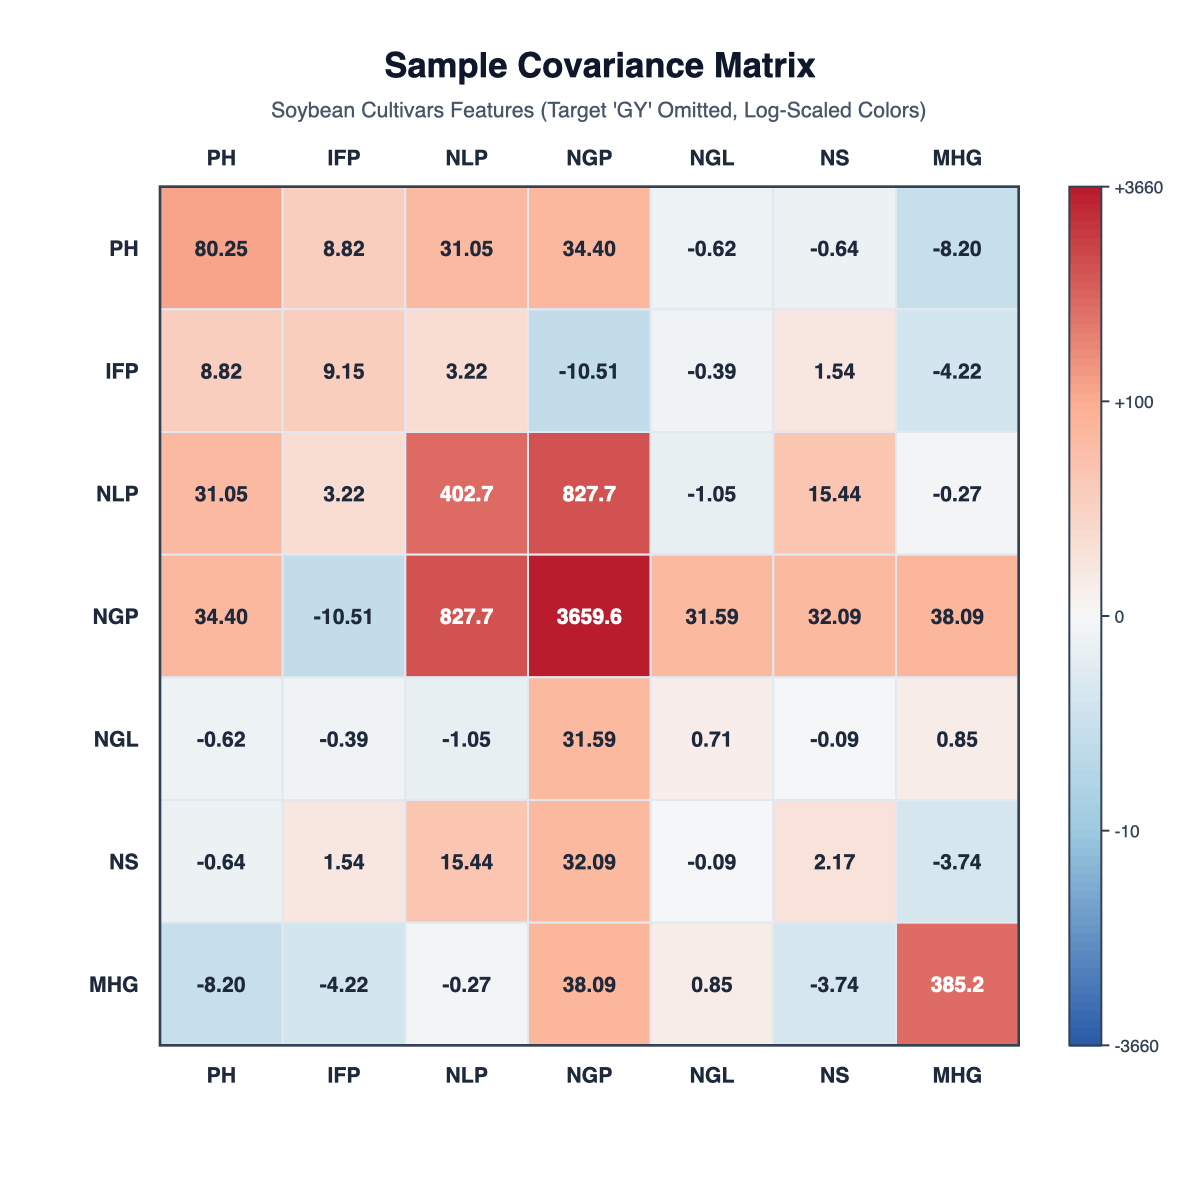
\includegraphics[width=0.68\textwidth]{covariance_matrix.png}
\caption{Heatmap of the sample covariance matrix.}
\label{fig:cov_matrix}
\end{figure}

\noindent
\textbf{Interpretation:} The total variance across all 7 variables is $\sum_{i=1}^7 s_i^2 = 4539.7587$. On its own, \texttt{NGP} accounts for $3659.5880 / 4539.7587 = 80.61\%$ of the total unscaled variance, followed by \texttt{NLP} ($8.87\%$) and \texttt{MHG} ($8.48\%$). The largest off-diagonal covariance also occurs between \texttt{NLP} and \texttt{NGP} ($\text{Cov} = 827.7090$).

\subsection{Eigenvalues Table and Explained Variability}

Table~\ref{tab:cov_eigen} details the eigenvalues ($\lambda_k$), the percentage of variance explained by each principal component, and the cumulative variance percentage for the covariance-based PCA.

\begin{table}[H]
\centering
\caption{Eigenvalues and explained variance for PCA on the Covariance Matrix.}
\label{tab:cov_eigen}
\begin{tabular}{lrrr}
\toprule
\textbf{Component} & \textbf{Eigenvalue ($\lambda_k$)} & \textbf{Explained Variance (\%)} & \textbf{Cumulative Variance (\%)} \\
\midrule
\textbf{PC1} & 3859.2795 & 85.01\% &  85.01\% \\
\textbf{PC2} &  385.6580 &  8.50\% &  93.51\% \\
\textbf{PC3} &  208.4685 &  4.59\% &  98.10\% \\
\textbf{PC4} &   76.7777 &  1.69\% &  99.79\% \\
\textbf{PC5} &    8.3209 &  0.18\% &  99.97\% \\
\textbf{PC6} &    1.1348 &  0.02\% & 100.00\% \\
\textbf{PC7} &    0.1193 &  0.00\% & 100.00\% \\
\midrule
\textbf{Total} & \textbf{4539.7587} & \textbf{100.00\%} & --- \\
\bottomrule
\end{tabular}
\end{table}

\noindent
\textbf{Answers to Assignment Questions (Covariance Matrix):}
\begin{itemize}
    \item \textbf{How many principal components should be used to account for:}
    \begin{itemize}
        \item \textbf{a) 90\% of the variability:} \textbf{2 principal components} (\texttt{PC1} and \texttt{PC2} account for \textbf{93.51\%}).
        \item \textbf{b) 95\% of the variability:} \textbf{3 principal components} (\texttt{PC1} to \texttt{PC3} account for \textbf{98.10\%}).
        \item \textbf{c) 99\% of the variability:} \textbf{4 principal components} (\texttt{PC1} to \texttt{PC4} account for \textbf{99.79\%}).
    \end{itemize}
    \item \textbf{Percentage of variability accounted for by the first two and first three PCs:}
    \begin{itemize}
        \item \textbf{First 2 principal components:} \textbf{93.51\%} ($85.01\% + 8.50\%$).
        \item \textbf{First 3 principal components:} \textbf{98.10\%} ($85.01\% + 8.50\% + 4.59\%$).
    \end{itemize}
\end{itemize}

\subsection{Scree Plot}

Figure~\ref{fig:cov_scree} displays the scree plot of individual and cumulative explained variance across all 7 components for the covariance matrix PCA.

\begin{figure}[H]
\centering
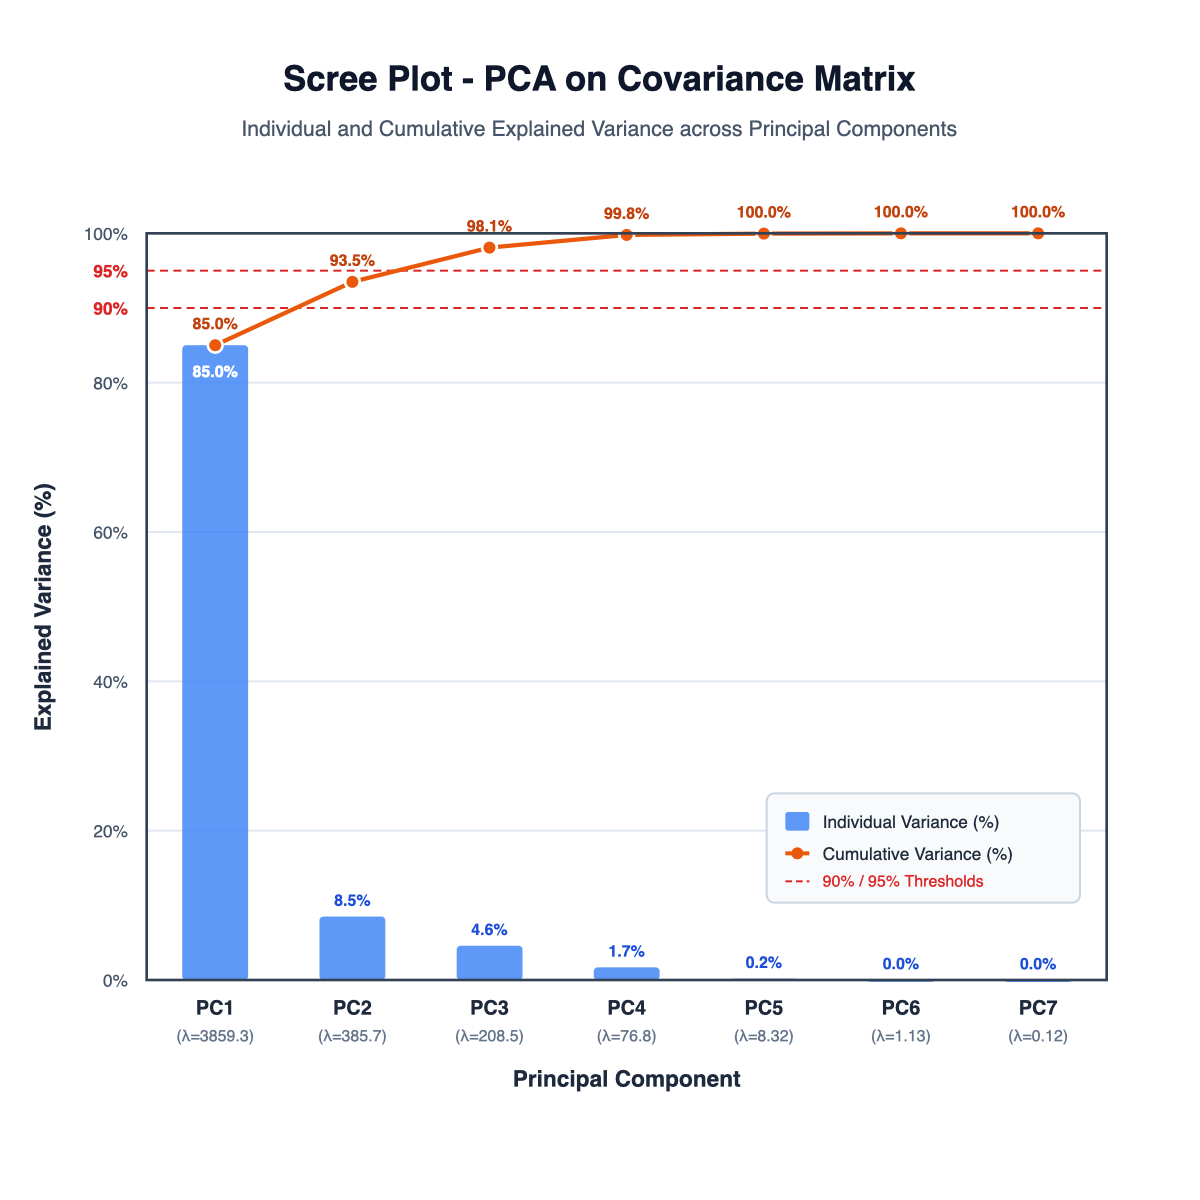
\includegraphics[width=0.72\textwidth]{cov_scree_plot.png}
\caption{Scree plot of individual and cumulative variance explained (Covariance Matrix).}
\label{fig:cov_scree}
\end{figure}

\noindent
\textbf{Interpretation:} The scree plot shows a very sharp drop after \texttt{PC1} ($85.01\% \rightarrow 8.50\%$). The cumulative curve crosses the $90\%$ threshold at \texttt{PC2} ($93.51\%$) and the $95\%$ threshold at \texttt{PC3} ($98.10\%$), while \texttt{PC5}--\texttt{PC7} contribute less than $0.25\%$ combined.

\subsection{Factor Loadings and Eigenvectors}

Table~\ref{tab:cov_eigvecs} presents the normalized eigenvectors $e_{ik}$ (the linear combination weights), and Table~\ref{tab:cov_loadings} reports the factor loadings $L_{ik} = \text{Corr}(X_i, \text{PC}_k) = \frac{e_{ik}\sqrt{\lambda_k}}{s_i}$, which measure the linear correlation between each original variable and each principal component.

\begin{table}[H]
\centering
\caption{Eigenvectors (linear combination weights $e_{ik}$) for the Covariance Matrix.}
\label{tab:cov_eigvecs}
\begin{tabular}{lrrrrrrr}
\toprule
\textbf{Variable} & \textbf{PC1} & \textbf{PC2} & \textbf{PC3} & \textbf{PC4} & \textbf{PC5} & \textbf{PC6} & \textbf{PC7} \\
\midrule
\texttt{PH}  &  0.0107 & -0.0325 &  0.1676 &  0.9780 & -0.1090 &  0.0485 &  0.0010 \\
\texttt{IFP} & -0.0024 & -0.0126 &  0.0341 &  0.1126 &  0.9676 & -0.2232 &  0.0022 \\
\texttt{NLP} &  0.2330 & -0.0561 &  0.9544 & -0.1687 & -0.0229 & -0.0376 &  0.0364 \\
\texttt{NGP} &  0.9723 &  0.0030 & -0.2311 &  0.0299 &  0.0070 & -0.0009 & -0.0172 \\
\texttt{NGL} &  0.0079 &  0.0027 & -0.0403 &  0.0065 & -0.0096 & -0.0349 &  0.9985 \\
\texttt{NS}  &  0.0090 & -0.0117 &  0.0342 & -0.0294 &  0.2262 &  0.9722 &  0.0377 \\
\texttt{MHG} &  0.0106 &  0.9977 &  0.0608 &  0.0233 &  0.0100 &  0.0082 & -0.0001 \\
\bottomrule
\end{tabular}
\end{table}

\begin{table}[H]
\centering
\caption{Factor loadings (correlations between variables and PCs) for the Covariance Matrix.}
\label{tab:cov_loadings}
\begin{tabular}{lrrrrrrr}
\toprule
\textbf{Variable} & \textbf{PC1} & \textbf{PC2} & \textbf{PC3} & \textbf{PC4} & \textbf{PC5} & \textbf{PC6} & \textbf{PC7} \\
\midrule
\texttt{PH}  &  0.0744 & -0.0712 &  0.2702 & \textbf{0.9566} & -0.0351 &  0.0058 &  0.0000 \\
\texttt{IFP} & -0.0502 & -0.0816 &  0.1627 &  0.3263 & \textbf{0.9229} & -0.0786 &  0.0002 \\
\texttt{NLP} & \textbf{0.7211} & -0.0549 & \textbf{0.6867} & -0.0737 & -0.0033 & -0.0020 &  0.0006 \\
\texttt{NGP} & \textbf{0.9985} &  0.0010 & -0.0552 &  0.0043 &  0.0003 &  0.0000 & -0.0001 \\
\texttt{NGL} & \textbf{0.5839} &  0.0624 & \textbf{-0.6921} &  0.0680 & -0.0330 & -0.0443 &  0.4104 \\
\texttt{NS}  &  0.3795 & -0.1564 &  0.3344 & -0.1746 &  0.4425 & \textbf{0.7024} &  0.0088 \\
\texttt{MHG} &  0.0336 & \textbf{0.9984} &  0.0447 &  0.0104 &  0.0015 &  0.0004 &  0.0000 \\
\bottomrule
\end{tabular}
\end{table}

\subsection{Equations of the First Three Principal Components}

Let $X'_i = X_i - \bar{X}_i$ denote the mean-centered variables. Using the eigenvector weights from Table~\ref{tab:cov_eigvecs}, the mathematical representations of the first three principal components are:
{\small
\begin{align}
\text{PC}_1 &= 0.0107\,\text{PH}' - 0.0024\,\text{IFP}' + 0.2330\,\text{NLP}' + 0.9723\,\text{NGP}' + 0.0079\,\text{NGL}' + 0.0090\,\text{NS}' + 0.0106\,\text{MHG}' \\
\text{PC}_2 &= -0.0325\,\text{PH}' - 0.0126\,\text{IFP}' - 0.0561\,\text{NLP}' + 0.0030\,\text{NGP}' + 0.0027\,\text{NGL}' - 0.0117\,\text{NS}' + 0.9977\,\text{MHG}' \\
\text{PC}_3 &= 0.1676\,\text{PH}' + 0.0341\,\text{IFP}' + 0.9544\,\text{NLP}' - 0.2311\,\text{NGP}' - 0.0403\,\text{NGL}' + 0.0342\,\text{NS}' + 0.0608\,\text{MHG}'
\end{align}
}

\subsection{2D and 3D Principal Component Plots}

Figures~\ref{fig:cov_2d} and \ref{fig:cov_3d} illustrate the 2D projection (\texttt{PC1} vs.\ \texttt{PC2}) and the 3D projection (\texttt{PC1}, \texttt{PC2}, \texttt{PC3}) of the 320 observations stratified by \texttt{Season}.

\begin{figure}[H]
\centering
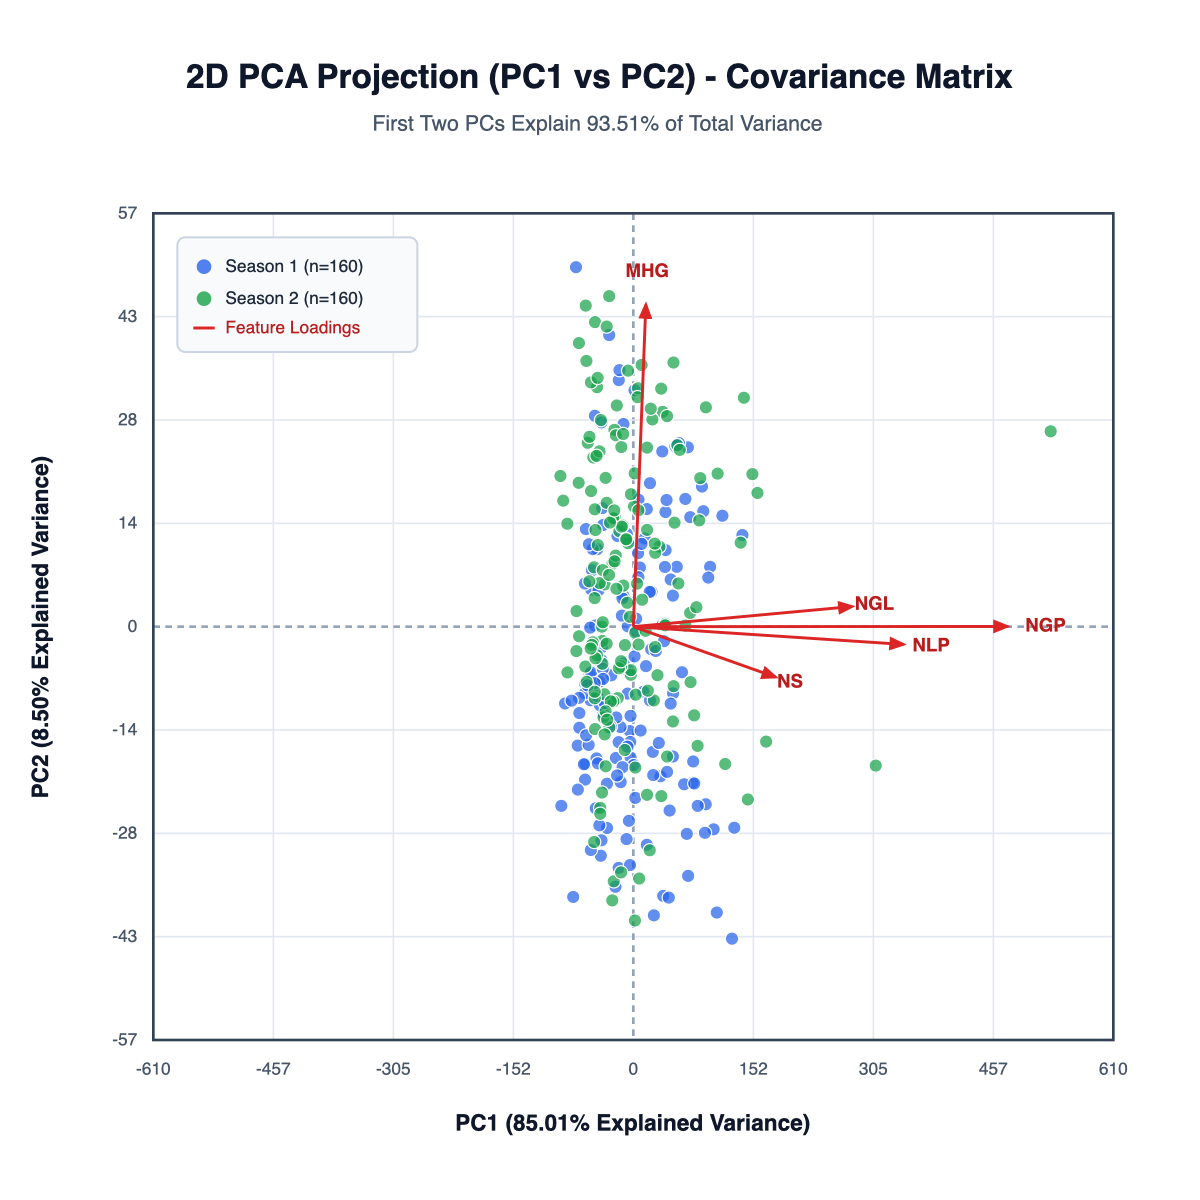
\includegraphics[width=0.72\textwidth]{cov_pca_2d.png}
\caption{2D graph of the first two principal components using the Covariance Matrix (93.51\% explained variance).}
\label{fig:cov_2d}
\end{figure}

\begin{figure}[H]
\centering
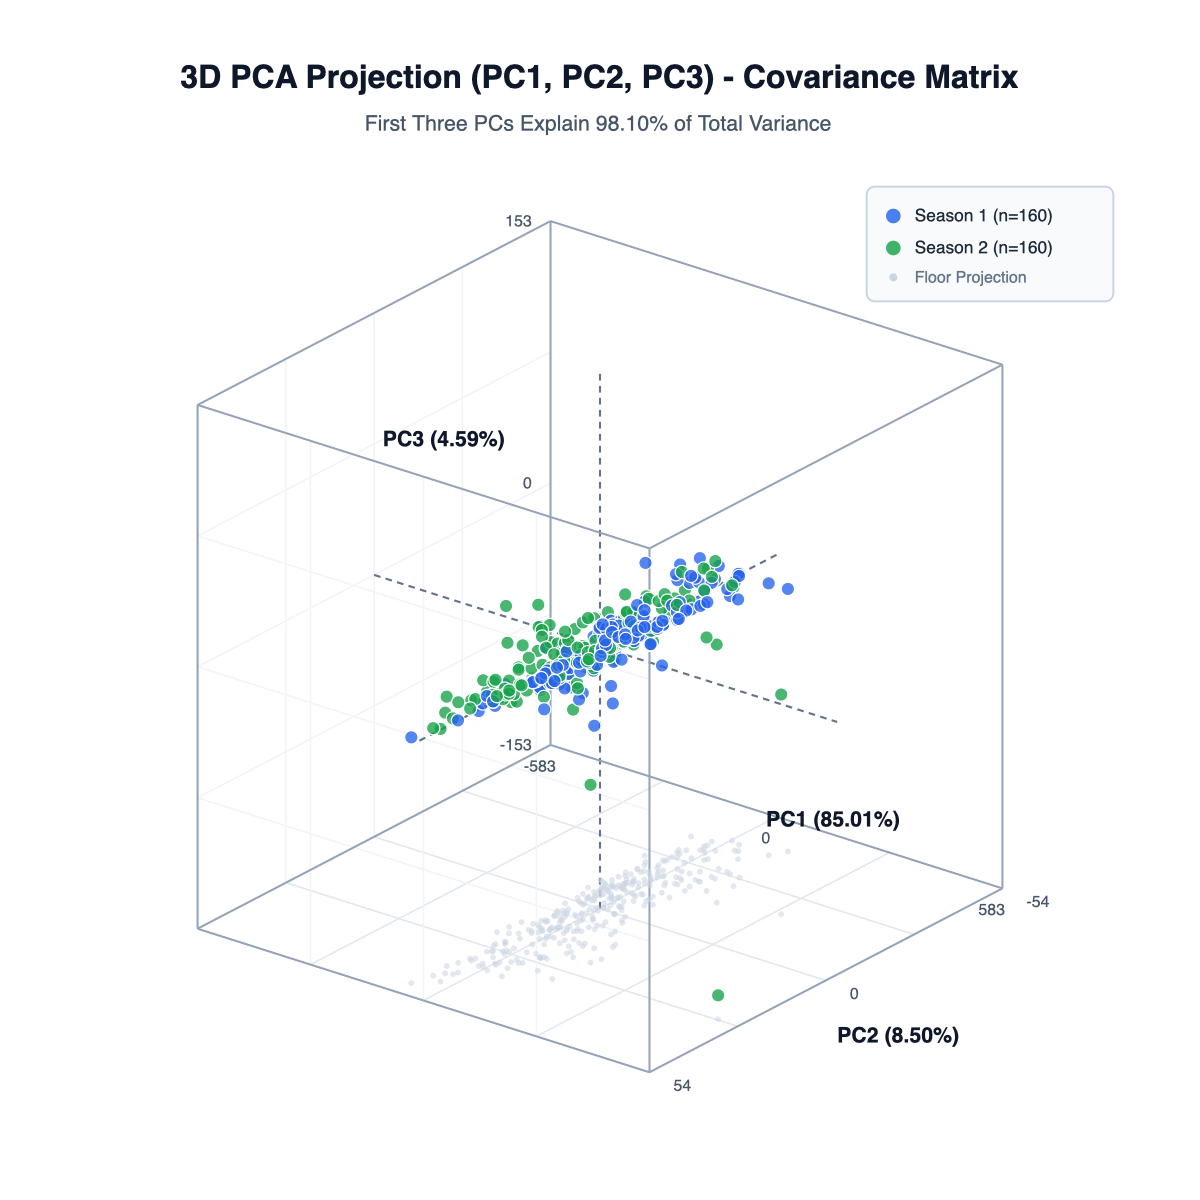
\includegraphics[width=0.72\textwidth]{cov_pca_3d.png}
\caption{3D graph of the first three principal components using the Covariance Matrix (98.10\% explained variance).}
\label{fig:cov_3d}
\end{figure}

\subsection{Description and Interpretation (Covariance Matrix PCA)}

\begin{enumerate}
    \item \textbf{Dominance of High-Magnitude Traits:} Because covariance PCA operates on unstandardized units, each component is pulled toward the variable with the largest numerical variance. \textbf{PC1 (85.01\%)} is almost identical to \texttt{NGP} (weight $0.9723$, factor loading $r = 0.9985$), while also correlating with \texttt{NLP} ($r = 0.7211$) and \texttt{NGL} ($r = 0.5839$) due to their biological association with total grain count.
    \item \textbf{Orthogonal Seed Weight Axis (\texttt{PC2}):} \textbf{PC2 (8.50\%)} has an eigenvector weight of $0.9977$ and a factor loading of $0.9984$ on \texttt{MHG} (Mass of 100 Grains). In Figure~\ref{fig:cov_2d}, the \texttt{MHG} loading arrow points straight up along the vertical \texttt{PC2} axis, completely perpendicular to the horizontal \texttt{NGP}/\texttt{NLP} axis.
    \item \textbf{Pod Count Contrast (\texttt{PC3}):} \textbf{PC3 (4.59\%)} is dominated by \texttt{NLP} (weight $0.9544$, loading $0.6867$) contrasted against \texttt{NGL} (loading $-0.6921$). Similarly, \texttt{PC4} ($1.69\%$) isolates Plant Height (\texttt{PH}, weight $0.9780$, loading $0.9566$). Thus, covariance PCA simply orders the individual variables from largest variance to smallest variance rather than extracting balanced multi-trait components.
\end{enumerate}

\section{PCA Using the Correlation Matrix}

\subsection{Correlation Matrix and Heatmap}

Standardizing the variables to zero mean and unit variance ($s_i^2 = 1.0$) yields the Pearson correlation matrix shown in Table~\ref{tab:corr_matrix} and visualized in Figure~\ref{fig:corr_matrix}.

\begin{table}[H]
\centering
\caption{Pearson correlation matrix (target variable \texttt{GY} omitted).}
\label{tab:corr_matrix}
\begin{tabular}{lrrrrrrr}
\toprule
 & \textbf{PH} & \textbf{IFP} & \textbf{NLP} & \textbf{NGP} & \textbf{NGL} & \textbf{NS} & \textbf{MHG} \\
\midrule
\textbf{PH}  &  1.0000 &  0.3254 &  0.1727 &  0.0635 & -0.0820 & -0.0487 & -0.0466 \\
\textbf{IFP} &  0.3254 &  1.0000 &  0.0531 & -0.0574 & -0.1516 &  0.3444 & -0.0711 \\
\textbf{NLP} &  0.1727 &  0.0531 &  1.0000 &  0.6818 & -0.0621 &  0.5219 & -0.0007 \\
\textbf{NGP} &  0.0635 & -0.0574 &  0.6818 &  1.0000 &  0.6215 &  0.3597 &  0.0321 \\
\textbf{NGL} & -0.0820 & -0.1516 & -0.0621 &  0.6215 &  1.0000 & -0.0736 &  0.0516 \\
\textbf{NS}  & -0.0487 &  0.3444 &  0.5219 &  0.3597 & -0.0736 &  1.0000 & -0.1293 \\
\textbf{MHG} & -0.0466 & -0.0711 & -0.0007 &  0.0321 &  0.0516 & -0.1293 &  1.0000 \\
\bottomrule
\end{tabular}
\end{table}

\begin{figure}[H]
\centering
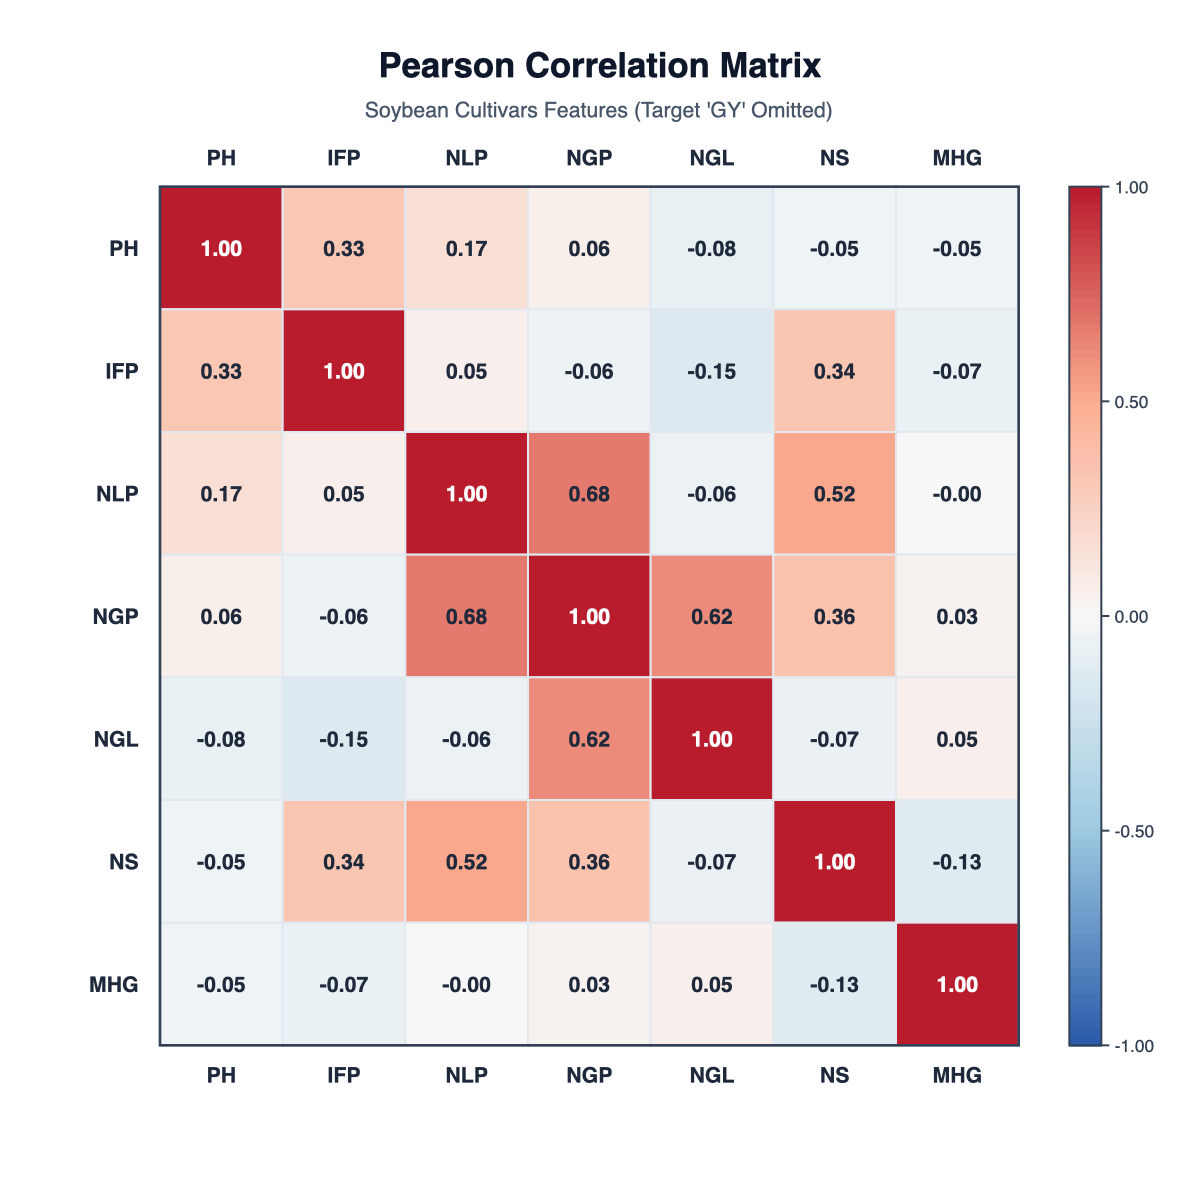
\includegraphics[width=0.68\textwidth]{correlation_matrix.png}
\caption{Heatmap of the Pearson correlation matrix.}
\label{fig:corr_matrix}
\end{figure}

\noindent
\textbf{Interpretation:} The correlation matrix highlights three strong positive relationships among reproductive traits: \texttt{NLP} and \texttt{NGP} ($r = 0.6818$), \texttt{NGP} and \texttt{NGL} ($r = 0.6215$), and \texttt{NLP} and \texttt{NS} ($r = 0.5219$). Moderate positive correlations also exist between \texttt{NS} and \texttt{NGP} ($r = 0.3597$), \texttt{IFP} and \texttt{NS} ($r = 0.3444$), and \texttt{PH} and \texttt{IFP} ($r = 0.3254$). Meanwhile, \texttt{MHG} shows near-zero correlations with all other features ($|r| \le 0.1293$).

\subsection{Eigenvalues Table and Explained Variability}

Table~\ref{tab:corr_eigen} summarizes the eigenvalues ($\lambda_k$), individual variance percentages, and cumulative variance percentages for the correlation-based PCA (where total standardized variance equals $7.0000$).

\begin{table}[H]
\centering
\caption{Eigenvalues and explained variance for PCA on the Correlation Matrix.}
\label{tab:corr_eigen}
\begin{tabular}{lrrr}
\toprule
\textbf{Component} & \textbf{Eigenvalue ($\lambda_k$)} & \textbf{Explained Variance (\%)} & \textbf{Cumulative Variance (\%)} \\
\midrule
\textbf{PC1} & 2.1666 & 30.95\% &  30.95\% \\
\textbf{PC2} & 1.6165 & 23.09\% &  54.04\% \\
\textbf{PC3} & 1.0712 & 15.30\% &  69.35\% \\
\textbf{PC4} & 0.9789 & 13.98\% &  83.33\% \\
\textbf{PC5} & 0.8147 & 11.64\% &  94.97\% \\
\textbf{PC6} & 0.3063 &  4.38\% &  99.35\% \\
\textbf{PC7} & 0.0458 &  0.65\% & 100.00\% \\
\midrule
\textbf{Total} & \textbf{7.0000} & \textbf{100.00\%} & --- \\
\bottomrule
\end{tabular}
\end{table}

\noindent
\textbf{Answers to Assignment Questions (Correlation Matrix):}
\begin{itemize}
    \item \textbf{How many principal components should be used to account for:}
    \begin{itemize}
        \item \textbf{a) 90\% of the variability:} \textbf{5 principal components} (\texttt{PC1} to \texttt{PC5} account for \textbf{94.97\%}).
        \item \textbf{b) 95\% of the variability:} \textbf{6 principal components} (\texttt{PC1} to \texttt{PC6} account for \textbf{99.35\%}).
        \item \textbf{c) 99\% of the variability:} \textbf{6 principal components} (\texttt{PC1} to \texttt{PC6} account for \textbf{99.35\%}).
    \end{itemize}
    \item \textbf{Percentage of variability accounted for by the first two and first three PCs:}
    \begin{itemize}
        \item \textbf{First 2 principal components:} \textbf{54.04\%} ($30.95\% + 23.09\%$).
        \item \textbf{First 3 principal components:} \textbf{69.35\%} ($30.95\% + 23.09\% + 15.30\%$).
    \end{itemize}
\end{itemize}

\subsection{Scree Plot}

Figure~\ref{fig:corr_scree} displays the scree plot for the correlation matrix PCA.

\begin{figure}[H]
\centering
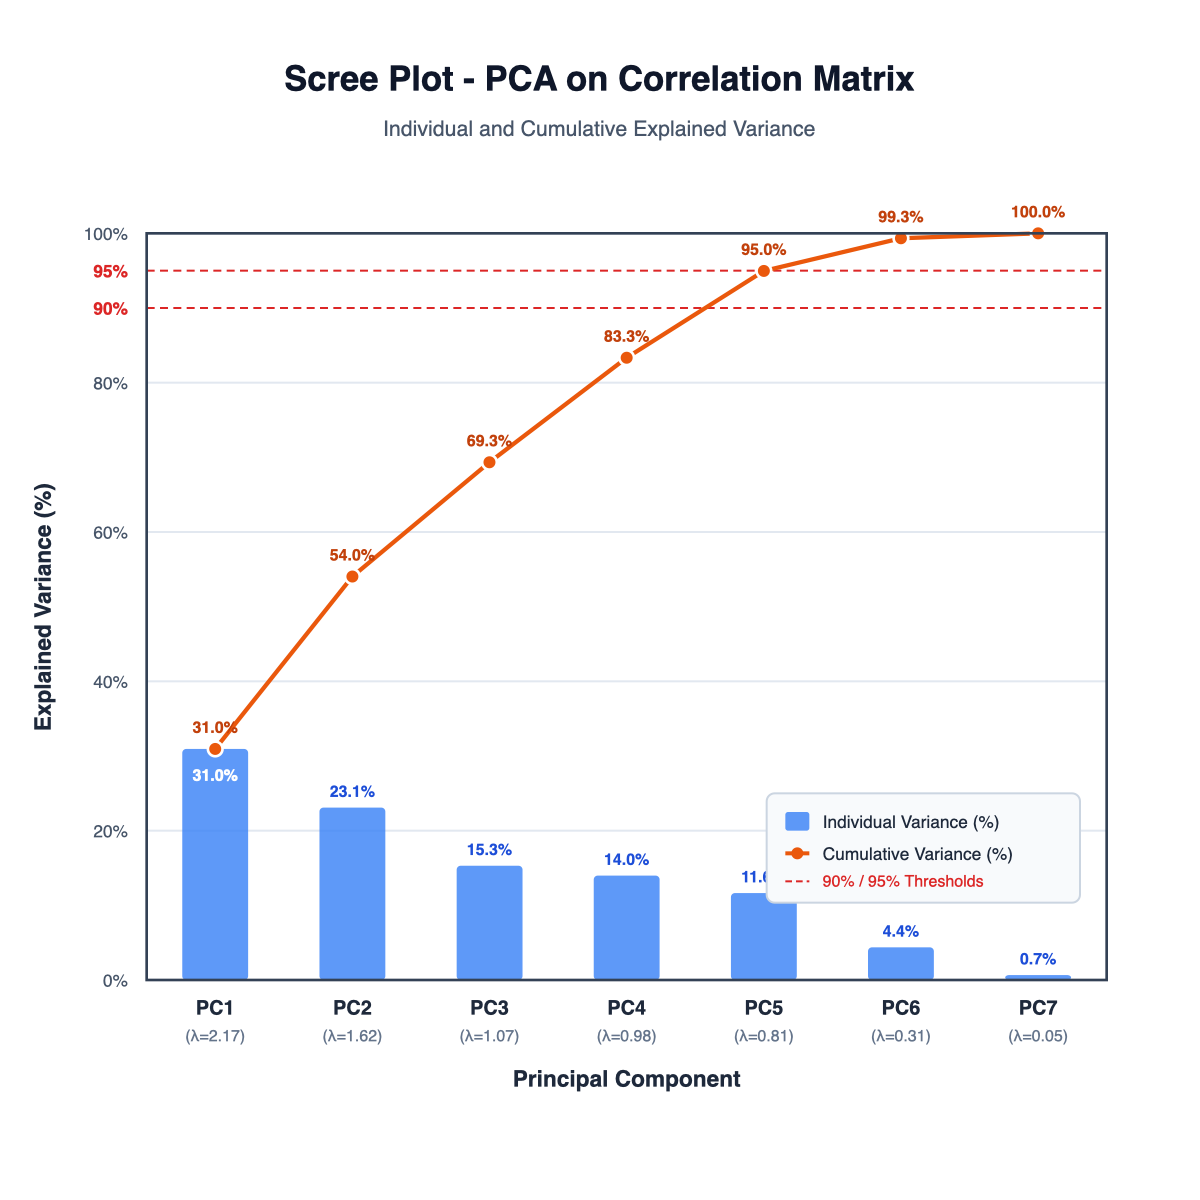
\includegraphics[width=0.72\textwidth]{corr_scree_plot.png}
\caption{Scree plot of individual and cumulative variance explained (Correlation Matrix).}
\label{fig:corr_scree}
\end{figure}

\noindent
\textbf{Interpretation:} Unlike the covariance scree plot, the explained variance is distributed across multiple components: \texttt{PC1} ($30.95\%$), \texttt{PC2} ($23.09\%$), \texttt{PC3} ($15.30\%$), \texttt{PC4} ($13.98\%$), and \texttt{PC5} ($11.64\%$). Under the Kaiser criterion ($\lambda_k > 1$), the first 3 components are retained (with \texttt{PC4} borderline at $\lambda_4 = 0.9789$). Furthermore, \texttt{PC7} has an eigenvalue close to zero ($\lambda_7 = 0.0458$, $0.65\%$) because \texttt{NGP} is structurally determined by \texttt{NLP} and \texttt{NGL} ($\text{NGP} \approx \text{NLP} \times \text{NGL}$), allowing 6 components to capture $99.35\%$ of total variance.

\subsection{Factor Loadings and Eigenvectors}

Table~\ref{tab:corr_eigvecs} presents the eigenvectors $e_{ik}$ and Table~\ref{tab:corr_loadings} reports the factor loadings $L_{ik} = e_{ik}\sqrt{\lambda_k}$ for the correlation matrix PCA.

\begin{table}[H]
\centering
\caption{Eigenvectors (linear combination weights $e_{ik}$) for the Correlation Matrix.}
\label{tab:corr_eigvecs}
\begin{tabular}{lrrrrrrr}
\toprule
\textbf{Variable} & \textbf{PC1} & \textbf{PC2} & \textbf{PC3} & \textbf{PC4} & \textbf{PC5} & \textbf{PC6} & \textbf{PC7} \\
\midrule
\texttt{PH}  &  0.1227 & -0.3560 &  0.7421 & -0.0686 & -0.3849 &  0.3932 &  0.0080 \\
\texttt{IFP} &  0.1412 & -0.5538 &  0.2700 & -0.0669 &  0.6209 & -0.4587 & -0.0053 \\
\texttt{NLP} &  0.5733 & -0.0990 & -0.1316 &  0.2479 & -0.4127 & -0.3701 & -0.5248 \\
\texttt{NGP} &  0.6016 &  0.3192 &  0.1175 & -0.0569 & -0.0366 & -0.1805 &  0.6966 \\
\texttt{NGL} &  0.2317 &  0.5682 &  0.3275 & -0.3465 &  0.3717 &  0.1373 & -0.4889 \\
\texttt{NS}  &  0.4682 & -0.2919 & -0.4052 &  0.0538 &  0.3032 &  0.6607 & -0.0107 \\
\texttt{MHG} & -0.0389 &  0.2163 &  0.2718 &  0.8962 &  0.2542 &  0.1003 &  0.0012 \\
\bottomrule
\end{tabular}
\end{table}

\begin{table}[H]
\centering
\caption{Factor loadings (correlations between variables and PCs) for the Correlation Matrix.}
\label{tab:corr_loadings}
\begin{tabular}{lrrrrrrr}
\toprule
\textbf{Variable} & \textbf{PC1} & \textbf{PC2} & \textbf{PC3} & \textbf{PC4} & \textbf{PC5} & \textbf{PC6} & \textbf{PC7} \\
\midrule
\texttt{PH}  &  0.1806 & -0.4526 & \textbf{0.7680} & -0.0679 & -0.3474 &  0.2176 &  0.0017 \\
\texttt{IFP} &  0.2078 & \textbf{-0.7042} &  0.2794 & -0.0662 & \textbf{0.5604} & -0.2539 & -0.0011 \\
\texttt{NLP} & \textbf{0.8439} & -0.1259 & -0.1362 &  0.2452 & -0.3725 & -0.2049 & -0.1123 \\
\texttt{NGP} & \textbf{0.8854} &  0.4059 &  0.1216 & -0.0563 & -0.0330 & -0.0999 &  0.1490 \\
\texttt{NGL} &  0.3411 & \textbf{0.7224} &  0.3389 & -0.3429 &  0.3355 &  0.0760 & -0.1046 \\
\texttt{NS}  & \textbf{0.6892} & -0.3711 & -0.4194 &  0.0532 &  0.2736 &  0.3657 & -0.0023 \\
\texttt{MHG} & -0.0573 &  0.2750 &  0.2813 & \textbf{0.8867} &  0.2295 &  0.0555 &  0.0003 \\
\bottomrule
\end{tabular}
\end{table}

\subsection{Equations of the First Three Principal Components}

Let $X^*_i = \frac{X_i - \bar{X}_i}{s_i}$ denote the standardized variables. Using the eigenvector weights from Table~\ref{tab:corr_eigvecs}, the mathematical representations of the first three principal components are:
\begin{align}
\text{PC}_1 &= 0.1227\,\text{PH}^* + 0.1412\,\text{IFP}^* + 0.5733\,\text{NLP}^* + 0.6016\,\text{NGP}^* + 0.2317\,\text{NGL}^* + 0.4682\,\text{NS}^* - 0.0389\,\text{MHG}^* \\
\text{PC}_2 &= -0.3560\,\text{PH}^* - 0.5538\,\text{IFP}^* - 0.0990\,\text{NLP}^* + 0.3192\,\text{NGP}^* + 0.5682\,\text{NGL}^* - 0.2919\,\text{NS}^* + 0.2163\,\text{MHG}^* \\
\text{PC}_3 &= 0.7421\,\text{PH}^* + 0.2700\,\text{IFP}^* - 0.1316\,\text{NLP}^* + 0.1175\,\text{NGP}^* + 0.3275\,\text{NGL}^* - 0.4052\,\text{NS}^* + 0.2718\,\text{MHG}^*
\end{align}

\subsection{2D and 3D Principal Component Plots}

Figures~\ref{fig:corr_2d} and \ref{fig:corr_3d} show the 2D projection (\texttt{PC1} vs.\ \texttt{PC2}) and the 3D projection (\texttt{PC1}, \texttt{PC2}, \texttt{PC3}) obtained from the correlation matrix PCA.

\begin{figure}[H]
\centering
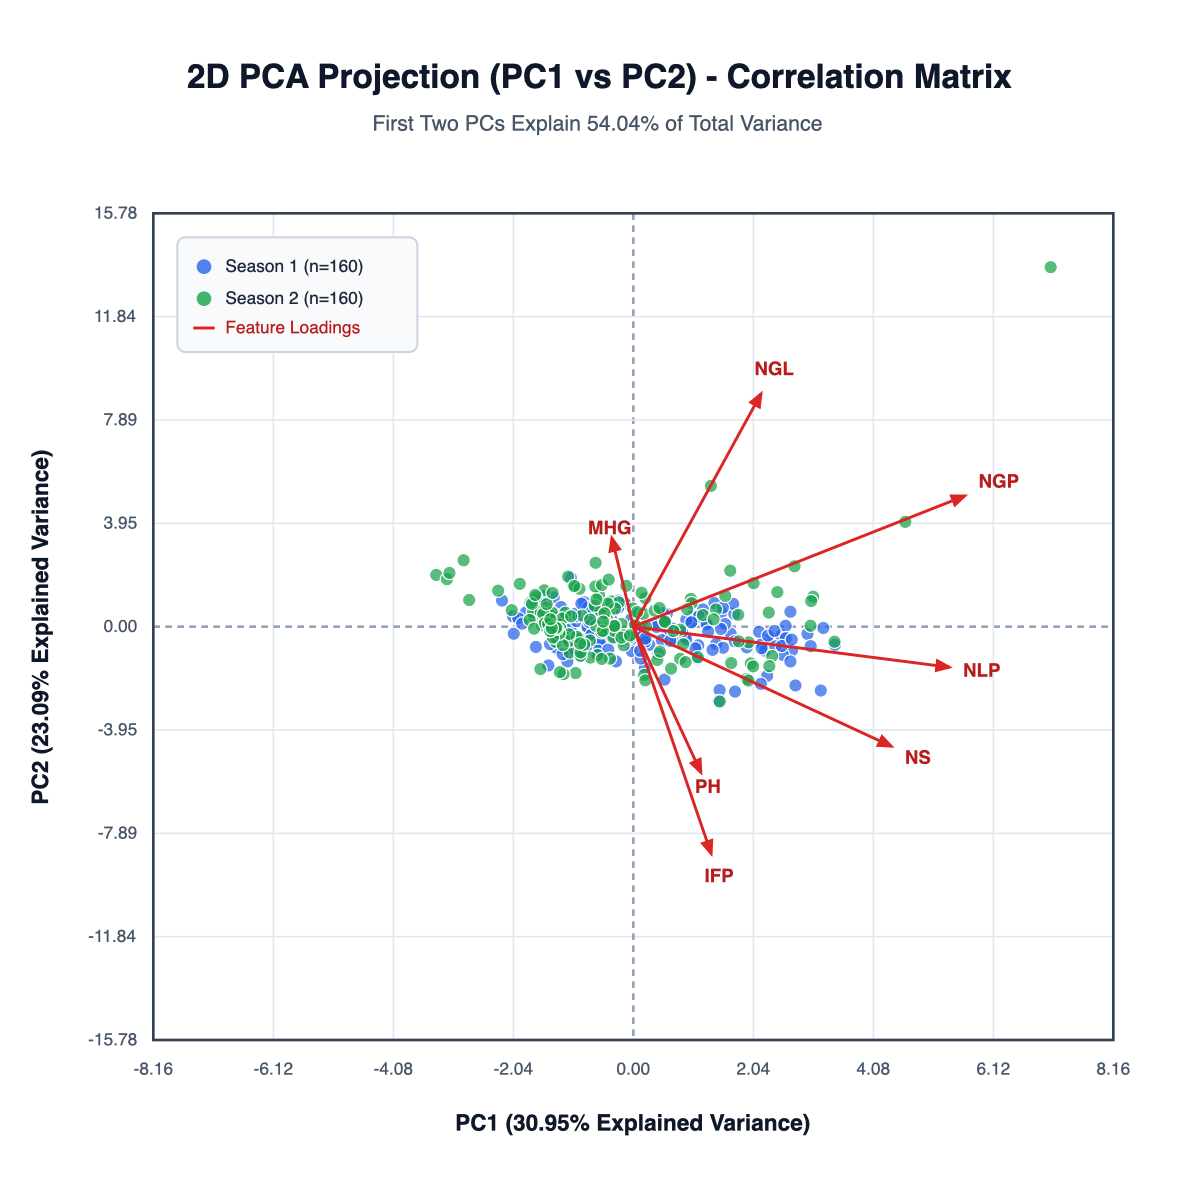
\includegraphics[width=0.72\textwidth]{corr_pca_2d.png}
\caption{2D graph of the first two principal components using the Correlation Matrix (54.04\% explained variance).}
\label{fig:corr_2d}
\end{figure}

\begin{figure}[H]
\centering
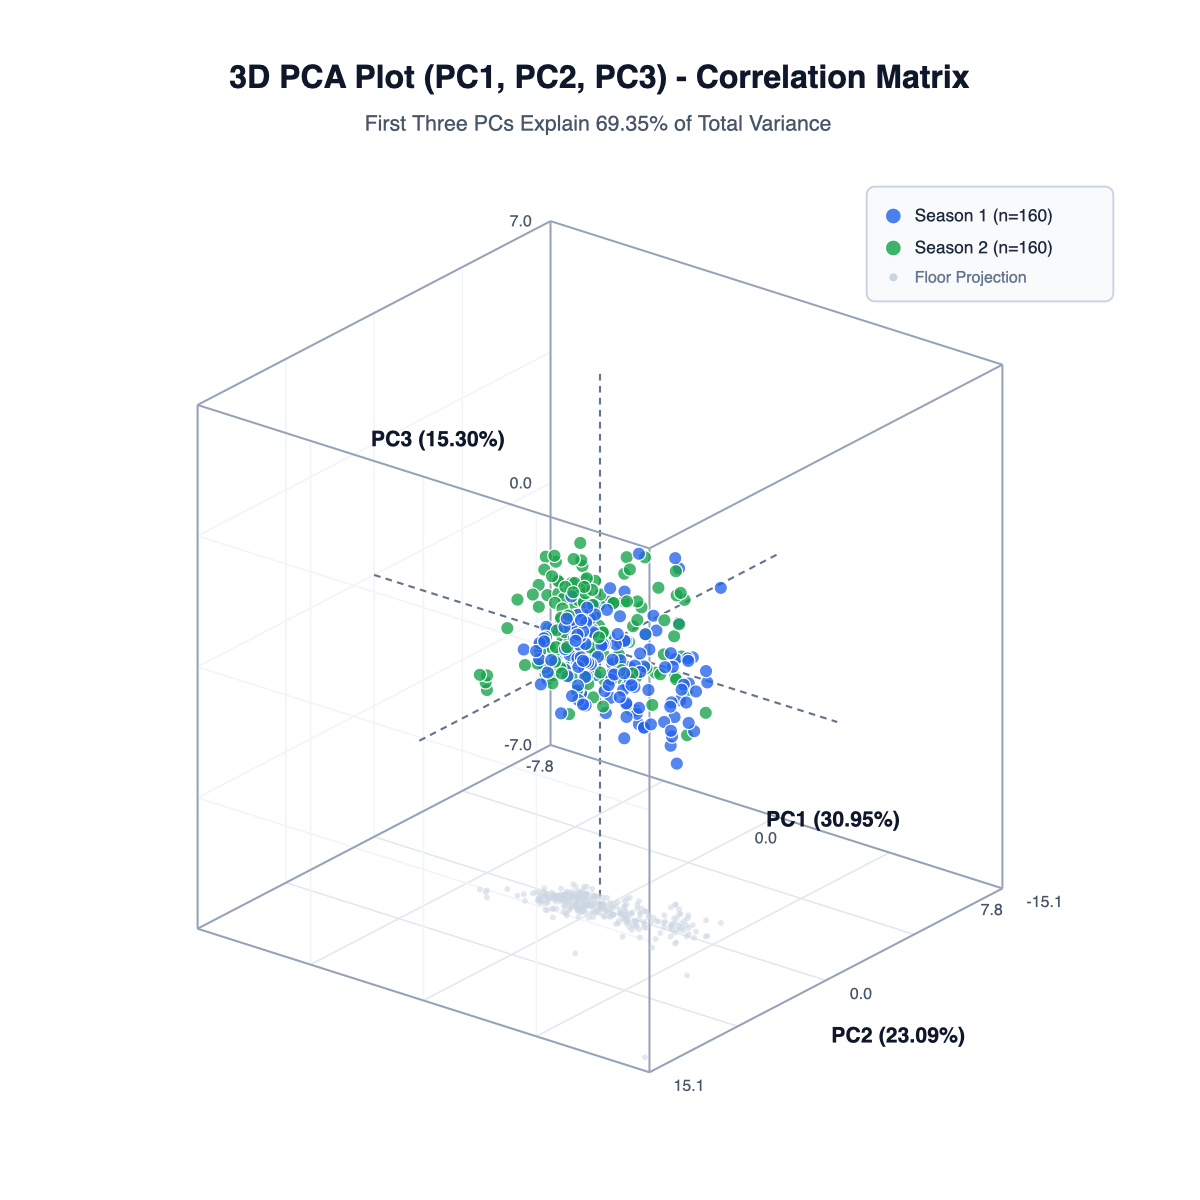
\includegraphics[width=0.72\textwidth]{corr_pca_3d.png}
\caption{3D graph of the first three principal components using the Correlation Matrix (69.35\% explained variance).}
\label{fig:corr_3d}
\end{figure}

\subsection{Description and Interpretation (Correlation Matrix PCA)}

\begin{enumerate}
    \item \textbf{PC1 -- Overall Plant Productivity and Branching (30.95\%):} \texttt{PC1} shows strong positive factor loadings with \texttt{NGP} ($0.8854$), \texttt{NLP} ($0.8439$), and \texttt{NS} ($0.6892$). Biologically, this axis represents the reproductive volume of the plant: plants with more stems (\texttt{NS}) develop more pods (\texttt{NLP}) and consequently more total grains (\texttt{NGP}). In Figure~\ref{fig:corr_2d}, Season~1 observations (blue) generally shift toward positive \texttt{PC1} values compared to Season~2 (green).
    \item \textbf{PC2 -- Pod Fertility vs.\ Structural Insertion Height (23.09\%):} \texttt{PC2} has a strong positive loading on \texttt{NGL} ($0.7224$) and \texttt{NGP} ($0.4059$), opposed by negative loadings on \texttt{IFP} ($-0.7042$), \texttt{PH} ($-0.4526$), and \texttt{NS} ($-0.3711$). It separates plants with high grain density per pod and lower pod insertion from taller plants with high first-pod insertion and fewer seeds per pod.
    \item \textbf{PC3 -- Vegetative Stature vs.\ Branching Architecture (15.30\%):} \texttt{PC3} is driven primarily by \texttt{PH} (loading $+0.7680$) against \texttt{NS} (loading $-0.4194$), distinguishing tall, single-stem plants from shorter, highly branched plants.
    \item \textbf{PC4 -- Independent Grain Weight Dimension (13.98\%):} \texttt{PC4} is dominated by \texttt{MHG} (loading $+0.8867$), confirming that hundred-grain weight behaves as an independent agronomic trait that does not covary linearly with pod or stem numbers.
\end{enumerate}

\section{Discussion of Results}

Table~\ref{tab:comparison} compares the key numerical results obtained from the two PCA approaches.

\begin{table}[H]
\centering
\caption{Comparison between Covariance Matrix PCA and Correlation Matrix PCA.}
\label{tab:comparison}
\begin{tabular}{lcc}
\toprule
\textbf{Criterion} & \textbf{a) Covariance Matrix PCA} & \textbf{b) Correlation Matrix PCA} \\
\midrule
Input transformation & Centered ($X - \bar{X}$) & Standardized ($(X - \bar{X})/s$) \\
Variance of first 2 PCs & 93.51\% (85.01\% + 8.50\%) & 54.04\% (30.95\% + 23.09\%) \\
Variance of first 3 PCs & 98.10\% (+ 4.59\%) & 69.35\% (+ 15.30\%) \\
PCs for $\ge 90\%$ variability & 2 PCs (93.51\%) & 5 PCs (94.97\%) \\
PCs for $\ge 95\%$ variability & 3 PCs (98.10\%) & 6 PCs (99.35\%) \\
PCs for $\ge 99\%$ variability & 4 PCs (99.79\%) & 6 PCs (99.35\%) \\
Primary drivers of PC1 & \texttt{NGP} ($r = 0.9985$) & \texttt{NGP} ($0.8854$), \texttt{NLP} ($0.8439$), \texttt{NS} ($0.6892$) \\
\bottomrule
\end{tabular}
\end{table}

\begin{enumerate}
    \item \textbf{Impact of Measurement Units and Scale Disparity:} In the covariance matrix PCA, the variance of \texttt{NGP} ($3659.59$) is more than 5,000 times larger than the variance of \texttt{NGL} ($0.71$). Consequently, the covariance eigenvalue decomposition attributes $85.01\%$ of the total variance to a single component (\texttt{PC1}) that nearly replicates \texttt{NGP}, while \texttt{PC2} ($8.50\%$) replicates \texttt{MHG} and \texttt{PC3} ($4.59\%$) replicates \texttt{NLP}. Small-scale traits (\texttt{NGL}, \texttt{NS}, \texttt{IFP}) receive negligible weights in the first three equations.
    \item \textbf{Superiority of Correlation Matrix PCA for Heterogeneous Traits:} Because our dataset combines variables with incompatible units (centimeters, counts, ratios, and grams), standardizing each variable to unit variance is essential. The correlation matrix PCA prevents high-count variables from monopolizing the components and reveals genuine multi-variable relationships.
    \item \textbf{Dimensionality and Collinearity Insight:} Even after standardization, the 7 features can be compressed to 6 components while retaining $99.35\%$ of the variance because \texttt{PC7} ($\lambda_7 = 0.0458$) reflects the multiplicative dependency $\text{NGP} \approx \text{NLP} \times \text{NGL}$. Meanwhile, the first three correlation components capture $69.35\%$ of the total standardized variance across three interpretable axes: reproductive capacity (\texttt{PC1}), pod fertility vs.\ insertion height (\texttt{PC2}), and plant stature vs.\ branching (\texttt{PC3}).
\end{enumerate}

\section{Conclusions}

\begin{itemize}
    \item \textbf{Covariance Matrix PCA:} The first two principal components explain \textbf{93.51\%} of the total variance and the first three explain \textbf{98.10\%}. To account for $90\%$, $95\%$, and $99\%$ of data variability, \textbf{2, 3, and 4 principal components} are required, respectively. However, these components are heavily biased by the raw numerical scale of \texttt{NGP}, \texttt{MHG}, and \texttt{NLP}.
    \item \textbf{Correlation Matrix PCA:} The first two principal components explain \textbf{54.04\%} of the total standardized variance and the first three explain \textbf{69.35\%}. To account for $90\%$, $95\%$, and $99\%$ of data variability, \textbf{5, 6, and 6 principal components} are required, respectively.
    \item \textbf{Methodological Recommendation:} For the \textit{Forty Soybean Cultivars} dataset, \textbf{PCA using the Correlation Matrix} is the appropriate method because the 7 agronomic predictors have different physical units and variances spanning four orders of magnitude. Correlation PCA balances the contribution of all variables and provides biologically meaningful latent factors for downstream modeling.
\end{itemize}

\end{document}
